\subsection*{NSC in the retina and visual cortex}

Due to its roots in efficient-coding theories of natural image processing,
\ac{NSC} figures prominently in the vision neuroscience literature.

For example, \ac{NMF}-based models were able to reconstruct
\emph{in vitro} neuronal spike trains from the salamander retina 
\cite{Onken2016,Liu2017}.
By combining spike-triggered average with \ac{NMF},
Liu and colleagues \cite{Liu2017} were able to identify the subunit layout
of retinal ganglion cells
(Fig.~\ref{fig:NMF|retina}).
\revise{This technique, termed \ac{STNMF},
involved applying \ac{NMF} to the collection of those stimulus patterns 
contained in a spatiotemporal white-noise sequence 
that caused a given neuron to spike.
Akin to common reverse-correlation analysis,
the researchers averaged the collection of spike-eliciting stimulus segments 
to form the spike-triggered stimulus ensemble (Fig.~\ref{fig:NMF|retina}A).
\Ac{STNMF} then decomposed the ensemble of effective spike-triggered stimuli into
a matrix \textbf{W} containing a set of modules (or basis functions)
and a matrix \textbf{H} containing a set of hidden coefficients.
% Whereas modules were constrained to have nonnegative elements,
% stimuli were represented by their contrast values (i.e., their relative deviation from mean light intensity, which could be positive or negative).
Intuitively, the modules derived by \ac{STNMF}
should capture the subunit decomposition of the cell's receptive field,
because the spike-eliciting stimuli should have essential statistical
structure imprinted on them by the subunits, such as correlations
between pixel values \cite{Liu2017}.}
And indeed, the identified \revise{modules} corresponded to 
individual presynaptic bipolar cells,
as verified by multielectrode array recordings with simultaneous recordings from
individual bipolar cells through sharp microelectrodes \cite{Liu2017}.
This allowed the researchers to improve predictions about how ganglion cells respond
to natural stimuli, without the need to guess a specific model structure that may be constrained in terms of the size, shape, number, or nonlinearity of 
ganglion cell subunits.

\begin{figure}[ht]
	\centering
	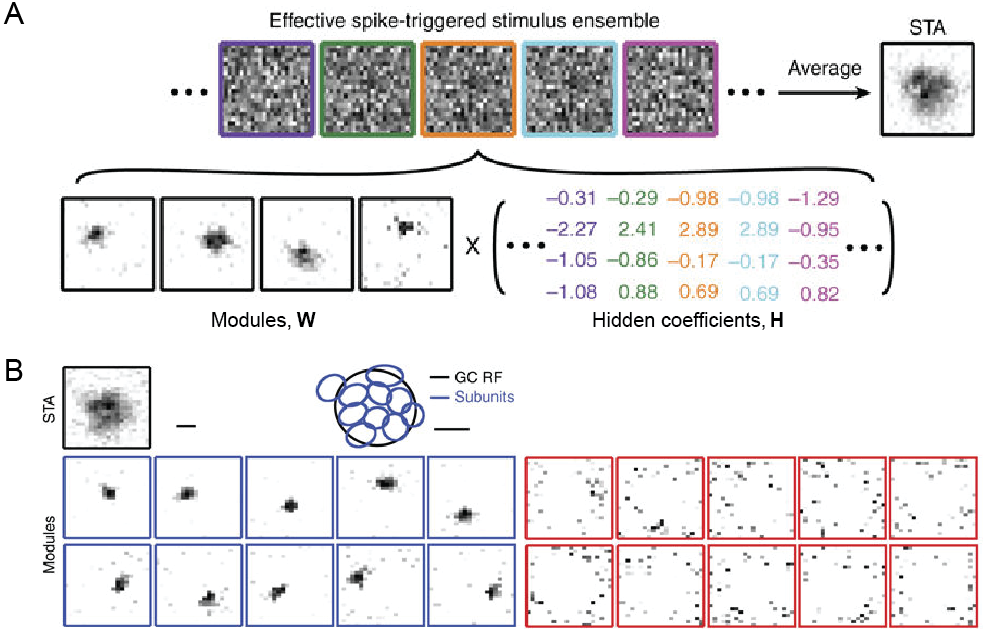
\includegraphics[width=\textwidth]{fig-rev2-retina}
    \caption{
    Identification of retinal ganglion cell subunits 
    with \ac{STNMF} (adapted \revise{with permission} from \cite{Liu2017}).
    \textbf{\emph{A}},
	     Samples of a ganglion cell’s effective spike-triggered stimulus ensemble (top),
         whose average corresponds to the cell’s \ac{STA}.
         For easier visual comparison with the subunits,
         \acp{STA} are displayed with negative pixel values set to zero and
         with zero corresponding to white in the grayscale image.
         \ac{STNMF} decomposes this ensemble into a set of modules and 
         \revise{hidden coefficients} (bottom).
         The example here shows four modules that were identified for
         a sample ganglion cell.
    \textbf{\emph{B}},
         Modules obtained for another sample ganglion cell by applying \ac{STNMF}
         with 20 modules (bottom 2 rows). Some modules have a strongly localized structure 
         (blue frames), others are more noise-like (red frames).
         \revise{These modules make up the subunits within a ganglion cell receptive field.}
         The top row shows the cell’s receptive field,
         given by the spatial component of the \ac{STA}, as well as the fitted \ac{RF} outline
         (GC RF, black ellipse), together with outlines of the localized subunits 
         (blue ellipses). Scale bars, 100 µm.
    }
	\label{fig:NMF|retina}
\end{figure}

As mentioned in the previous section,
\ac{NSC} has been extensively applied to early visual cortex,
where it has successfully explained 
orientation and frequency tuning of simple and complex cells in \ac{V1} \cite{Hoyer2003},
edge-like pooling of spatial frequency channels in V2 \cite{Hyvarinen2005},
including \ac{RF} properties such as end-stopping and contour integration 
\cite{HoyerHyvarinen2002}.
With the exception of face processing in \ac{IT}
\cite{LeeSeung1999,ChangTsao2017},
\ac{NSC} has yet to be applied to higher-order areas in the ventral visual stream.
The success of \ac{NSC} in explaining V1 and V2 response properties
suggests that it might be possible to extend the model to texture integration in
V4.

In our own work, we found evidence for \ac{NSC} in the dorsal visual stream.
Specifically, we demonstrated that simulated neurons 
in a \ac{NSC} based model of \ac{MSTd} 
responded to  large optic flow fields in much the same way as real neurons in macaque \ac{MSTd} \cite{Beyeler2016}.
Fig.~\ref{fig:NMF|MSTd} shows the distribution of direction preferences
of \ac{MSTd} cells (Fig.~\ref{fig:NMF|MSTd}A, B; \cite{Takahashi2007})
and \ac{MSTd}-like model units (Fig.~\ref{fig:NMF|MSTd}C, D; \cite{Beyeler2016})
for \revise{rotation and translation, respectively}.
Each data point in the scatter plots specifies the preferred 3D direction
of a single neuron or model unit.
Histograms along the boundaries show the marginal distributions of azimuth
and elevation preferences.
Not only did individual units match response properties of individual neurons
in macaque \ac{MSTd},
but the model was able to recover statistical properties of the \ac{MSTd}
population as a whole, such as a relative overrepresentation of lateral
headings (Fig.~\ref{fig:NMF|MSTd}C, D).

\begin{figure}[ht]
	\centering
	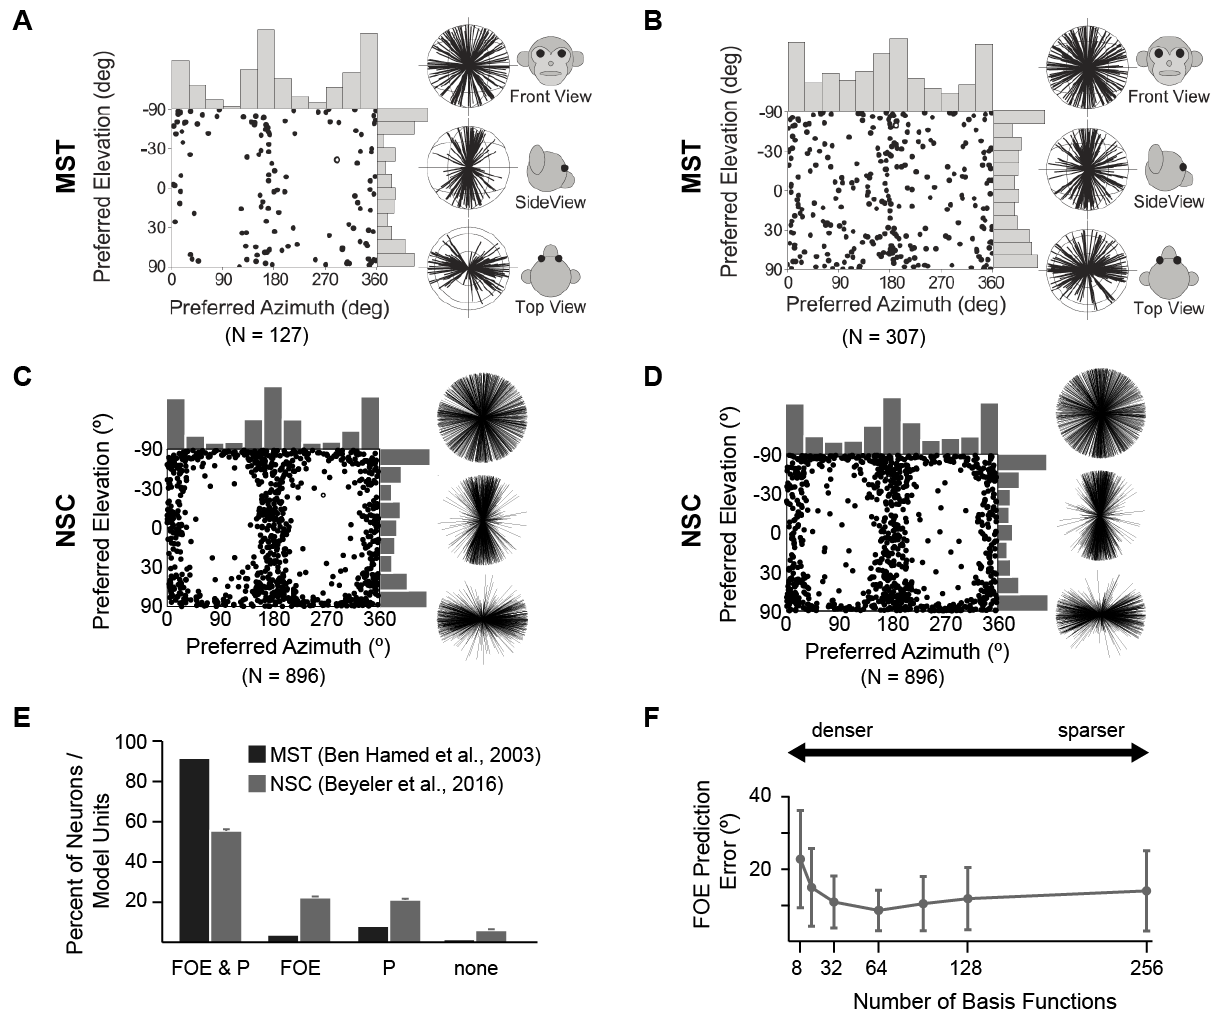
\includegraphics[width=0.95\textwidth]{fig-rev1-MST}
    \caption{
    \textbf{\emph{A-D}},
         Distribution of 3D direction preferences of macaque \ac{MSTd} neurons
         (rotation, \textbf{\emph{A}}; translation, \textbf{\emph{B}}; 
         reprinted \revise{with permission} from \cite{Takahashi2007})
         and model units in the \ac{NSC}-based sparse decomposition model
         (rotation, \textbf{\emph{C}}; translation, \textbf{\emph{D}}; 
         reprinted \revise{with permission} from \cite{Beyeler2016}).
         Each data point in the scatter plots corresponds to the preferred azimuth
         (abscissa) and elevation (ordinate) of a single neuron.
         Histograms along the top and right sides of each scatter plot show the
         marginal distributions.
         Also shown are 2D projections (front view, side view, and top view)
         of unit-length 3D preferred direction vectors (each radial line represents
         one neuron).
    \textbf{\emph{E}},
         Distribution of focus of expansion (FOE) and pursuit (P) selectivities
         in macaque \ac{MSTd} (dark gray) and model \ac{MSTd} (light gray;
         reprinted \revise{with permission} from \cite{Beyeler2016}).
         Neurons or model units were involved in encoding heading (FOE),
         eye velocity (P), both (FOE \& P), or neither (none).
    \textbf{\emph{F}},
         Heading prediction (generalization) error as a function of the
         number of basis functions using cross-validation.
         Vertical bars are the SD (reprinted \revise{with permission}
         from \cite{Beyeler2016}).
    }
	\label{fig:NMF|MSTd}
\end{figure}

\ac{MSTd} is known to encode a number of perceptual variables,
such as the direction of travel (heading) and eye rotation velocity.
During forward movement, retinal flow radiates out symmetrically from a single point,
the focus of expansion (FOE), from which heading can be inferred.
However, instead of consisting of a set of distinct subpopulations,
each specialized to encode a particular perceptual variable,
\ac{MSTd} has been found to consist of neurons that act more like basis functions,
where a majority of cells were involved in the simultaneous encoding of multiple
perceptual variables (Fig.~\ref{fig:NMF|MSTd}E).
A similar picture emerged when we investigated the involvement of \ac{MSTd}-like
model units in the encoding of both heading and eye rotation velocity
(Fig.~\ref{fig:NMF|MSTd}E).

Interestingly, the sparsity regime in which model \ac{MSTd} achieved the
lowest heading prediction error (Fig.~\ref{fig:NMF|MSTd}F) was also the
regime in which \ac{MSTd}-like model units reproduced a variety of known
\ac{MSTd} visual response properties
(for experimental details refer to \cite{Beyeler2016}).
\revise{In contrast to findings about early visual cortex,
this regime does not use an overcomplete basis set \cite{OlshausenField1996},
yet can still be considered a sparse coding regime \cite{SpanneJorntell2015},
since only a few \ac{MSTd}-like model units were needed to recover the stimulus,
and each model unit responded to a subset of stimuli (see Fig.~8C in \cite{Beyeler2016}).
Such an intermediary sparse code might be better suited
(as opposed to an overcomplete basis set)
for areas such as \ac{MSTd},
because the increased memory capacity of such a code might lead to compact
and multifaceted encodings of various perceptual variables.}


\subsection*{NSC in the auditory cortex}

The auditory cortex is a prime example of efficient coding. The auditory system is believed to decompose auditory signals into
a set of elementary acoustic features \cite{SmithLewicki2006},
such that the complete acoustic waveform can be described by a
sparse population code that operates near an information-theoretic optimum
\cite{SmithLewicki2006,rokem2006,Hromadka2008}.
It is therefore not surprising that computational models based on \ac{NSC}
have been very successful at describing the spectro-temporal \acp{RF}
of neurons in the \ac{A1} \cite{Martinez2015,David2007}.
Response properties of \ac{A1} neurons are well described by a spectrogram;
they are often tuned to stimulus frequency but are rarely phase-locked
to oscillations of the sound waveform \cite{Leaver2010}.
The cortical representation of auditory signals seems to not only be sparse,
but also rely on statistically independent acoustic features \cite{Klein2003}.

Similar to visual cortex, auditory cortex is hierarchically organized,
with neurons in \ac{A1} responding to simple acoustic features of natural sounds,
and higher-order areas responding to more behaviorally relevant stimuli.
The anterior superior temporal region of auditory cortex, for example,
responds to categories of acoustic objects,
such as sounds produced by voices and musical instruments
\cite{Leaver2010}.
An intriguing question for future modeling studies is therefore 
whether \ac{NSC} can be extended to the next level of the auditory hierarchy:
Would it be possible to construct more complex acoustic objects from a sparse,
parts-based set of elementary, \ac{A1}-like acoustic features?
And would the representation of such acoustic objects resemble neuronal responses
in the anterior superior temporal region of auditory cortex?


\subsection*{NSC in the olfactory cortex}

In contrast to most other sensory modalities, 
the basic perceptual dimensions of olfaction remain unclear.
Odors evoke complex responses in granule cells (located in the olfactory bulb)
that evolve over hundreds of milliseconds \cite{Broome2006}.
Granule cells use a sparse combinatorial code to convey information about odor identity
and concentration \cite{Koulakov2011,Gupta2015}.
Downstream from the olfactory bulb, odors tend to activate a small but consistent
proportion ($\sim 10\%$) of cortical neurons in the piriform cortex \cite{poo2009},
which is thought to form odor object percepts \cite{chen2014,stettler2009}.
Although piriform cortex is not topographically organized,
a spatial structure can be discerned when examining the projections of output neurons,
which are highly segregated and functionally specific.
Whereas the anterior piriform cortex is associated with the encoding of 
odor identity and odor structure, 
the posterior piriform cortex is involved in associational aspects of odors, 
such as valence and similarity \cite{chen2014,gottfried2006}.

\begin{figure}[b!]
	\centering
	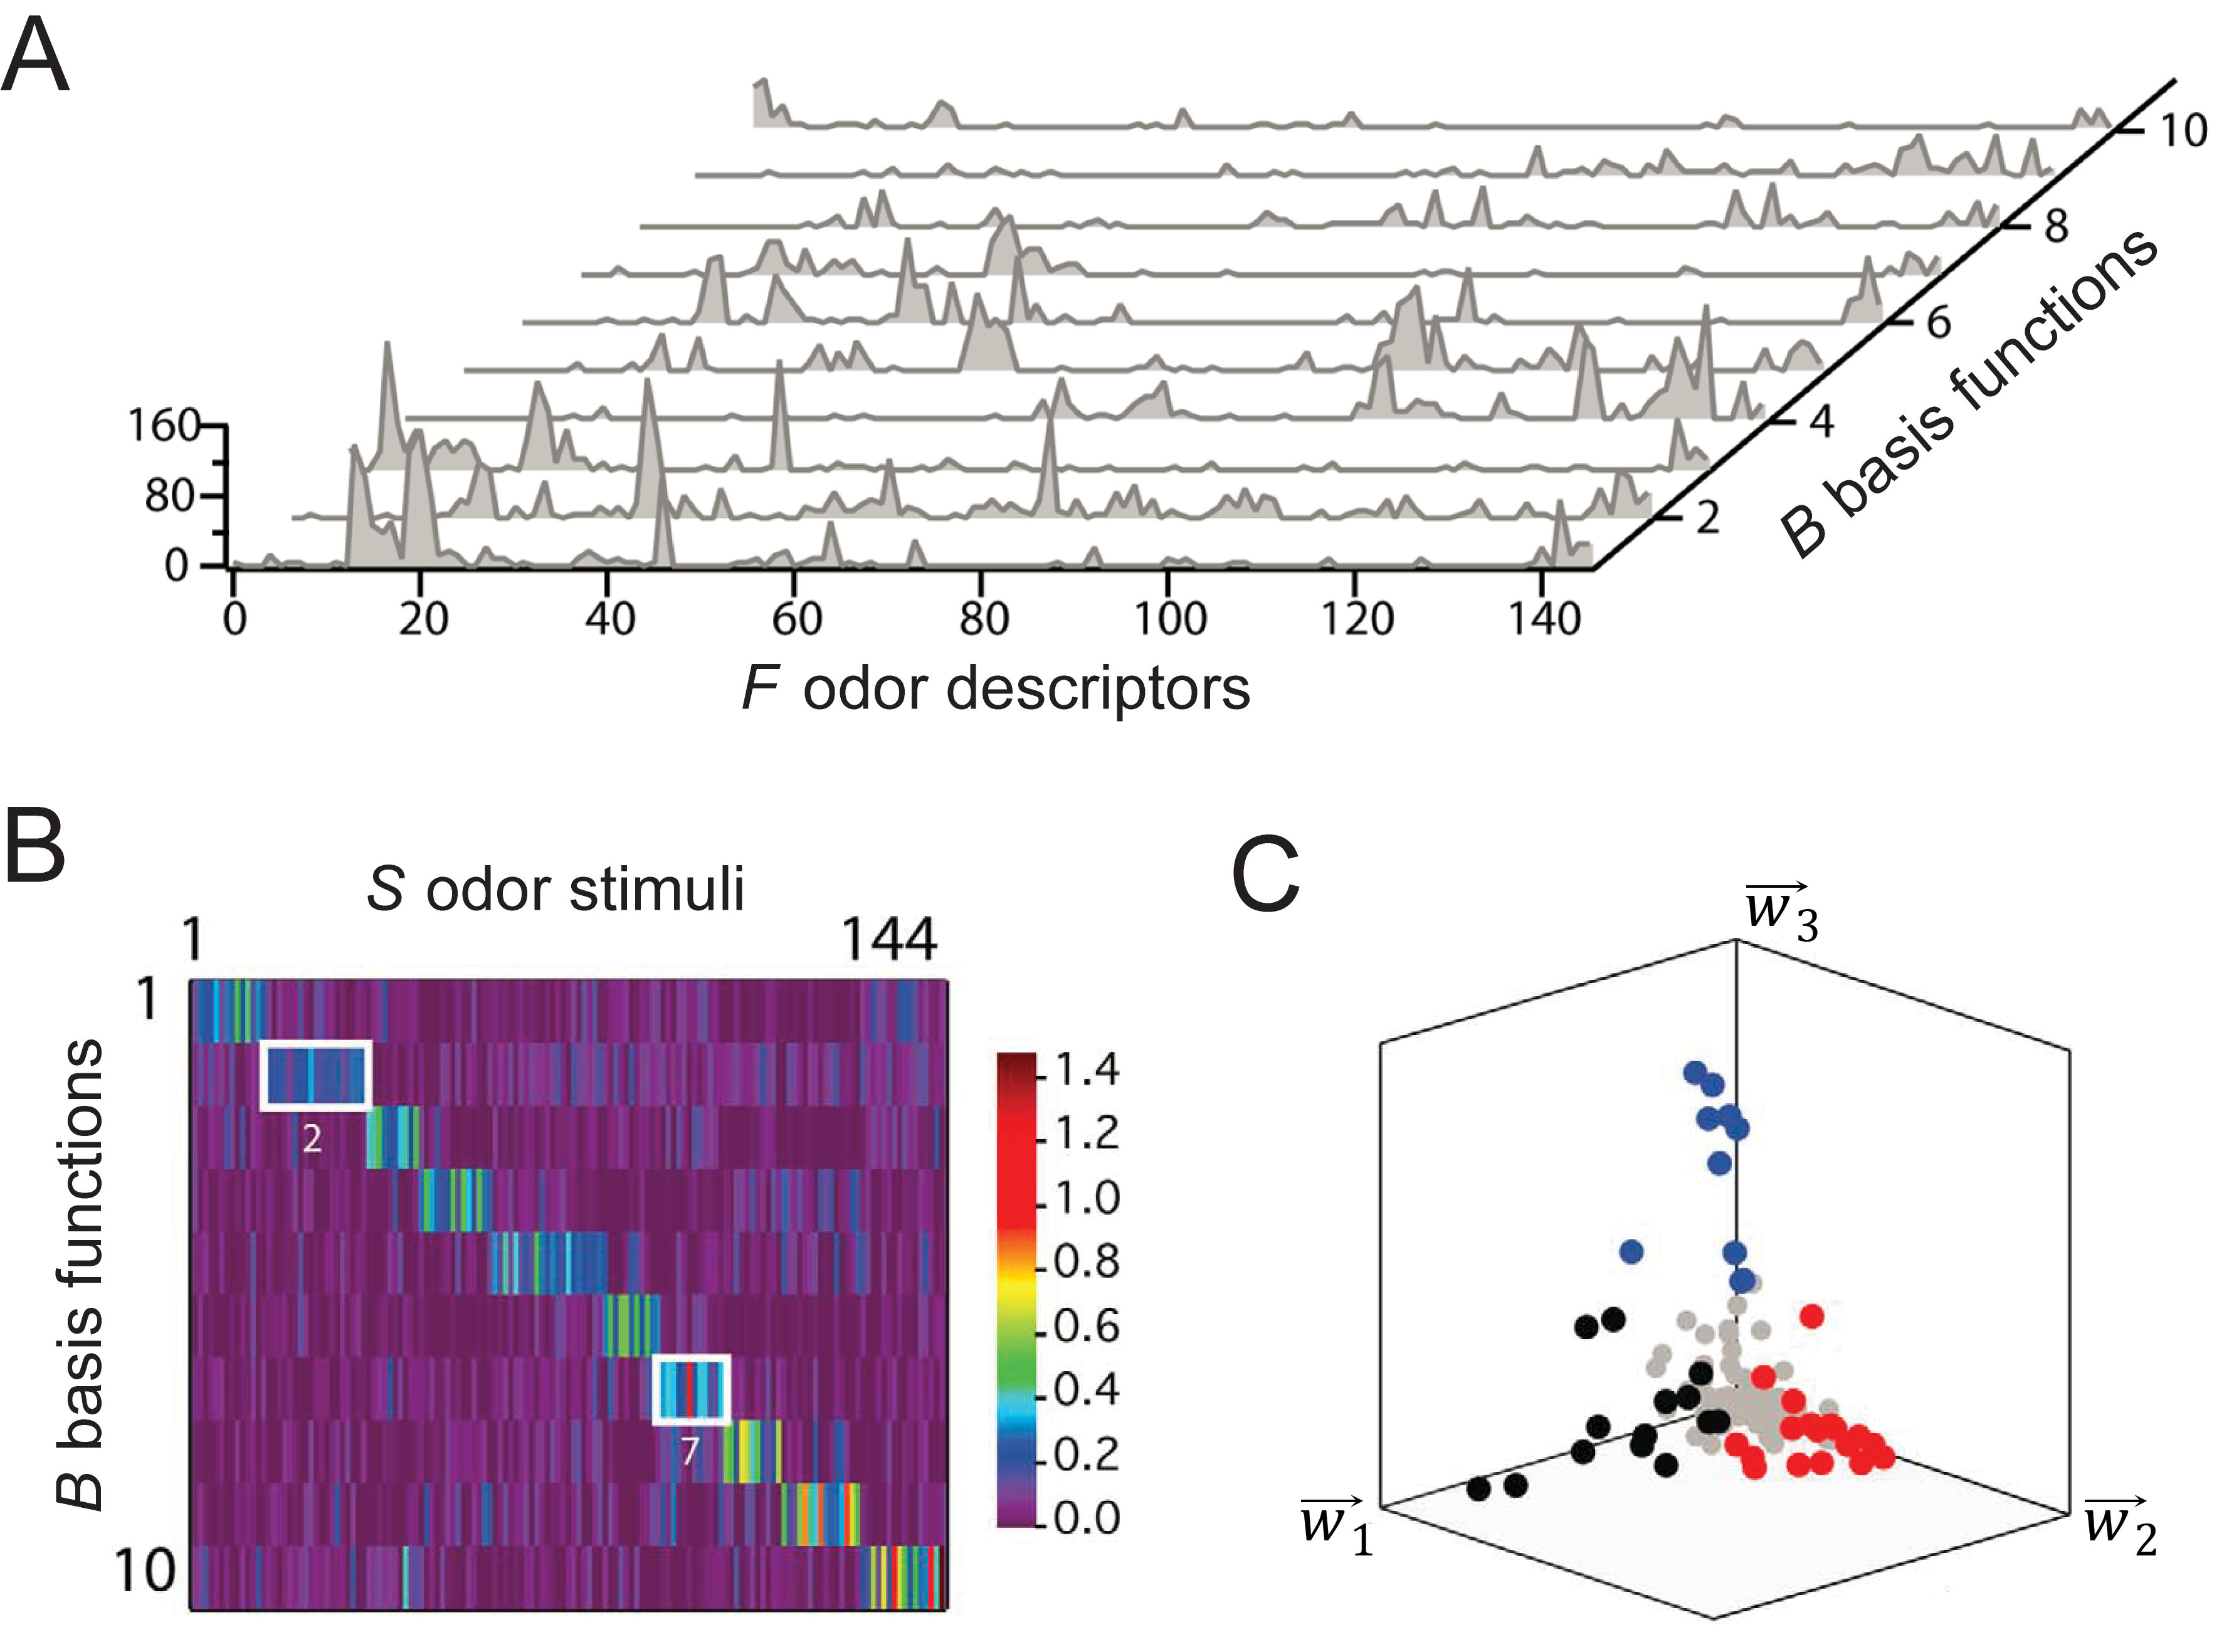
\includegraphics[width=0.95\textwidth]{fig-rev2-olfaction}
    \caption{\ac{NMF} recovers a sparse and parts-based representation
    of olfactory perceptual space (adapted \revise{with permission} 
    from \cite{Castro2013}).
       \textbf{\emph{A}},
          Waterfall plot of the 10 basis functions constituting \textbf{W}
          \revise{(same nomenclature as in Fig.~\ref{fig:NMF|reconstruction}).}
       \textbf{\emph{B}},
          Heat map of the \revise{hidden} coefficient matrix, \textbf{H},
          where each column of \textbf{H} corresponds to a different odor.
          Columns of \textbf{H} are normalized and sorted.
       \textbf{\emph{C}},
          Plot of all 144 odors in the dataset (each point is a column in \textbf{H})
          in the space spanned by the first three basis functions,
          \revise{$\vec{w_1}$ (`fragrant'/`floral'), 
          $\vec{w_2}$ (`woody, resinous'/`musty,earthy'), 
          and $\vec{w_3}$ (`fruity, other than citrus'/`sweet')}.
          Black, red, and blue points are those with 
          \revise{their largest hidden coefficient corresponding to the first,
          second, and third basis function}, respectively. 
          Gray points are all remaining odors.}
	\label{fig:evidence-olfaction}
\end{figure}

Castro and colleagues \cite{Castro2013} provided 
one of the most compelling pieces of evidence for \ac{NSC}
in the olfactory system to date:
In an effort to elucidate the dimensions along which perceptual space might be
organized in the olfactory system,
they applied \ac{NMF} to a dataset of 144 monomolecular odors,
each represented by a 146-dimensional \revise{vector (an `odor profile')}.
Each dimension in the odor profile corresponded to the rated applicability of
a number of semantic labels, such as `sweet', `floral', and `heavy'.
By applying \ac{NMF} to the odor profile, they showed that 
\revise{a total of 10} sparsely active set of basis functions 
could accurately describe any odor in the dataset
\revise{(Fig.~\ref{fig:evidence-olfaction}A)}.
Interestingly, \ac{NMF} revealed a prominent block
diagonal structure to the full matrix \textbf{H}
\revise{(Fig.~\ref{fig:evidence-olfaction}B)}, indicating that:
1) a given odor tended to be characterized by a single prominent \revise{basis function},
implying that the basis functions recovered by \ac{NMF} were perceptually meaningful,
and 2) all ten \revise{basis functions were being used approximately with equal frequency},
implying that the basis functions recovered by \ac{NMF} could span the space of
behaviorally relevant odors.
This suggests that a given odor percept may be considered an 
instance of one of several fundamental qualities.
% For the data set investigated, individual odor profiles were well-classified 
% by their proximity to a single one of these \revise{basis functions}, 
% with all ten \revise{basis functions} being approximately equally expressed 
% across the set of odors.

Furthermore, \ac{NMF} recovered basis functions whose descriptors aligned
with perceptual dimensions highlighted in several previous analyses of odor space,
including but not limited to relative pleasantness (e.g., `fragrant`, `sickening`), 
and potential palatability (`woody, resinous', `chemical', `sweet', and `lemon').
Odors clustered predominantly along these axes,
\revise{as illustrated in Fig.~\ref{fig:evidence-olfaction}C) for three
specific basis functions} \cite{Castro2013}.


\subsection*{NSC in the somatosensory cortex}
Of all of the sensory areas,
somatosensory cortex is among the best understood in terms of circuitry,
yet least understood in terms of sensory function
\cite{Ramirez2014}.
Spatiotemporal receptive fields indicate that 
\revise{some neurons respond to a small number of stimulus dimensions
(not unlike to sensory neurons in the visual system
\cite{Pei2008,Pei2011,DiCarlo1998}),
suggesting a possible role for dimensionality reduction
in \ac{S1} \cite{Ramirez2014}.}
\revise{However, tactile information from various submodalities converges
at the level of \ac{S1} \cite{HyvarinenPoranen1978,Pei2009}
and is multiplexed across different time scales 
using both rate and spike timing codes \cite{Harvey2013},
thus complicating any interpretation of the neural representation of touch
in these areas.}

In an effort to elucidate the stimulus dimensions that 
individual \revise{\ac{S1}} neurons respond to,
Whiteway and Butts \cite{WhitewayButts2017} devised the \ac{RLVM},
a combination of nonlinear dimensionality reduction with nonnegativity constraints
that is closely related to \ac{NSC}.
When they applied the \ac{RLVM} to 
a two-photon imaging dataset of hundreds of simultaneously recorded neurons 
in mouse primary somatosensory cortex while the animal was performing
a tactile discrimination task,
they found basis functions that properly identified individual neurons.
Similar to the recorded neuronal responses, these basis functions were closely related
to both the tactile stimulation as well as 
nonstimulus aspects of the behavioral task.
Furthermore, \ac{RLVM} achieved a lower reconstruction error than other
linear dimensionality reduction techniques such as \textbf{\ac{PCA}}.

Similar to auditory cortex,
activity in \revise{rodent} somatosensory cortex can be extremely sparse
\cite{Jadhav2009,oconnor2010,Crochet2011},
and sparse coding models have successfully explained the response properties
of individual neurons in rat somatosensory cortex (e.g., \cite{Hafner2004}).
% In addition, the presence of a topographically organized sensory `homunculus' 
% in various species \cite{penfield1937,hari1993,petersen2007} 
% suggests a possible parts-based representation scheme.
\revise{However, this finding might not generalize across species.
For example, London and Miller \cite{LondonMiller2013} found that
neurons in the proprioceptive arm area of macaque \ac{S1}
respond to movements in many directions,
which argues against sparse activity in this area.}


\subsection*{NSC in the retrosplenial cortex (RSC)}

In our own work, we found evidence that \ac{NSC} 
can explain response properties in \ac{RSC}, 
an area important for navigation and spatial memory 
\cite{Miller2014,Nelson2015,VannAggleton2009}.
Using a similar methodology to \cite{Beyeler2016},
we applied \ac{NMF}, with a sparsity constraint,
to parameterized behavioral variables extracted from electrophyisiological recordings
of \ac{RSC} neurons in the rat \cite{AlexanderNitz2015}
while the animal ran back and forth a W-shaped track
(for experimental details, see Supplementary Material).
As mentioned above, these behavioral variables included the animal's position, head direction, 
and movement direction (Fig.~\ref{fig:NMF|reconstruction}C).
The basis functions recovered by \ac{NMF} were then used to generate simulated responses
of model \ac{RSC} neurons according to Eq.~\ref{eqn:nsc-model-response},
and the simulated responses were compared to neuronal responses 
from the electrophysiological recordings.

We found that the population activity of these simulated neurons could be used to predict
the animal's location both with respect to the beginning of the route
(route-based reference frame)
and with respect to where the route was located within the room
(allocentric reference frame).
In addition, simulated neuronal activity could be classified into three broad categories,
with remarkably similar population statistics to rat \ac{RSC}:
1) responding to left and right turns on a specific position along the route,
2) responding to left and right turns regardless the position along the route,
and 3) exhibiting complex and robust firing patterns without turn sensitivity
(see Supplementary Material; also Fig.~\ref{fig:NMF|RSC}A, B).


\subsection*{Reinforcement-driven NSC in the basal ganglia}

There is computational evidence 
for a reward-driven variant of \ac{NSC} in the basal ganglia, 
a cluster of deep forebrain nuclei that are involved in the 
processing of motor, associative, and limbic information
(for recent reviews see \cite{BarGad2003_Review,NelsonKreitzer2014}).
The basal ganglia connect most cortical areas to the frontal cortex through
a series of convergent and sparsely connected pathways \cite{schwab2015},
where signals from tens of millions of cortical neurons are projected
onto a $10 - 10,000$ fold smaller population of neurons in different subnuclei
of the basal ganglia \cite{BarGad2003_Review}.

The \ac{RDDR} model suggests that dimensionality reduction 
in the cortico-basal ganglia pathway is achieved via
a combination of Hebbian and anti-Hebbian learning rules
that are implemented by feedforward excitatory and lateral inhibitory
connections \cite{BarGad2000,BarGad2003_Review}.
\revise{These learning rules control the strength of synaptic weights in the network 
by altering the weight of a given synapse in proportion to
the correlation between the firing rates of its presynaptic and postsynaptic neurons.
In Hebbian learning, synaptic weights are strengthened given a positive correlation 
(leading to a phenomenon referred to as long-term potentiation, or LTP),
while synaptic weights are depressed if the firing rate correlation is negative
(leading to as long-term depression, or LTD). On the other hand, in anti-Hebbian learning, which is typically applied to inhibitory connections, correlated activities are subjected to LTD and uncorrelated activities are subjected to LTP.
\jeffNote{This is my understanding of anti-Hebb. Make sure it applies to their model.}
In order to implement dopamine-modulated Hebbian learning in this model,
a reinforcement signal was used to dictate the level of dopamine in the circuit 
(1 for reward-related events, 0 for the absence of reward-related events, 
and negative values to simulate dopamine depletion) \cite{BarGad2000}.
The value of the reinforcement signal then determined the sign and magnitude
of each synaptic weight change.}

In the \ac{RDDR} model, a reinforcement signal corresponding to dopamine 
modulates the Hebbian learning rule of the feedforward projections,
allowing the network to learn to extract input dimensions
that are associated with reward activity
while suppressing behaviorally irrelevant input dimensions.
Whereas the original \ac{RDDR} model was a neural-network based model
for performing \ac{PCA} \cite{BarGad2000},
later iterations incorporated nonnegativity constraints on the
connection weights that effectively transformed the model 
into an \ac{NMF} variant \cite{BarGad2003_Review}.
\revise{The model predicted that these lateral connections facilitated learning
by shaping correlations between neurons in the corticostriatal projections
using dopamine-modulated LTP and LTD, which was later experimentally validated
\cite{calabresi2007dopamine}.}

% \revise{The ac{RDDR} model made two critical predictions, 
% one of which has yet to be tested experimentally. 
% First, this model was initially developed to explain the existence of the extensive inhibitory lateral connectivity found within the basal ganglia, which seem to have no functional purpose based on experimental data\emilyNote{clunky sentence, revise}. The RDDR model predicts that these connections facilitate learning and must thus be studied during the learning phase of a task either in young animals or in animals being exposed to a new environment. At this time, the lateral connections should show increased strength and the firing patterns of the connected neurons should be correlated. After learning, these connections are expected to rapidly lose efficacy. Second, at the time, Hebbian and anti-Hebbian learning modulated by a dopaminergic reinforcement signal had yet to be documented in the basal ganglia. However, since publication this prediction has been confirmed, as studies have revealed dopamine-modulated LTP and LTD as mechanisms that facilitate learning in corticostriatal synapses \cite{calabresi2007dopamine}.}
% \mikeNote{Compressed this paragraph into the above sentence.}

In addition to suggesting a role for lateral connectivity
in the basal ganglia,
the \ac{RDDR} model also advanced understanding of basal ganglia dysfunction
in movement-related disorders such as Parkinon's and Huntington's disease.
\revise{Previous studies had indicated that lesions to functionally healthy basal ganglia
had minimal impact on behavior. Bar-Gad and colleagues \cite{BarGad2000} then
suggested that this was an expected finding 
because of the network's ability to reorganize connections,
whereas abnormal dopamine levels should significantly alter 
the reinforcement signal that controls the model's ability 
to discriminate behaviorally relevant input signals (as in Parkinson's disease).
Accordingly, restoration of background dopamine levels via dopamine replacement therapy 
alleviate the symptoms, consistent with results of dopamine depletion and restoration 
in the model.}

% \emilyNote{While working on this, I found another Bar-Gad article that talks about somatotopic organization in the BG corresponding to face, arms, legs, etc, which may or may not be useful to bring up re: parts-based coding. https://www.frontiersin.org/articles/10.3389/fnsys.2011.00038/full}
% \mikeNote{Let's leave it here for the next round of revisions ^^ but so far the reviewers didn't have a problem with this section}
